\documentclass[a4paper,UTF8]{article}
\usepackage{ctex}
\usepackage[margin=1.25in]{geometry}
\usepackage{color}
\usepackage{graphicx}
\usepackage{amssymb}
\usepackage{amsmath}
\usepackage{amsthm}
\usepackage{enumerate}
\usepackage{bm}
\usepackage{hyperref}
\usepackage{float}
\numberwithin{equation}{section}
%\usepackage[thmmarks, amsmath, thref]{ntheorem}
\theoremstyle{definition}
\newtheorem*{solution}{Solution}
\newtheorem*{prove}{Proof}
\usepackage{multirow}

%--

%--
\begin{document}
\title{机器学习导论\\
习题四}
\author{151250104, 卢以宁, kiwiloveskiwis@gmail.com}
\maketitle
\section{\textbf{[20pts]} Reading Materials on CNN}
卷积神经网络(Convolution Neural Network,简称CNN)是一类具有特殊结构的神经网络,在深度学习的发展中具有里程碑式的意义。其中,Hinton于2012年提出的\href{https://en.wikipedia.org/wiki/AlexNet}{AlexNet}可以说是深度神经网络在计算机视觉问题上一次重大的突破。

关于AlexNet的具体技术细节总结在经典文章\href{https://papers.nips.cc/paper/4824-imagenet-classification-with-deep-convolutional-neural-networks}{“ImageNet Classification with Deep Convolutional Neural Networks”}, by Alex Krizhevsky, Ilya Sutskever and Geoffrey E. Hinton in NIPS'12,目前已逾万次引用。在这篇文章中,它提出使用ReLU作为激活函数,并创新性地使用GPU对运算进行加速。请仔细阅读该论文,并回答下列问题(请用1-2句话简要回答每个小问题,中英文均可)。

\begin{enumerate}[(a)]
\item \textbf{[5pts]} Describe your understanding of how ReLU helps its success? And, how do the GPUs help out?

\item \textbf{[5pts]} Using the average of predictions from several networks help reduce the error rates. Why?
\item \textbf{[5pts]} Where is the dropout technique applied? How does it help? And what is the cost of using dropout?
\item \textbf{[5pts]} How many parameters are there in AlexNet? Why the dataset size(1.2 million) is important for the success of AlexNet?
\end{enumerate}

关于CNN,推荐阅读一份非常优秀的学习材料,由南京大学计算机系吴建鑫教授\footnote{吴建鑫教授主页链接为\url{cs.nju.edu.cn/wujx}}所编写的讲义Introduction to Convolutional Neural Networks\footnote{由此链接可访问讲义\url{https://cs.nju.edu.cn/wujx/paper/CNN.pdf}},本题目为此讲义的Exercise-5,已获得吴建鑫老师授权使用。
\begin{solution}
此处用于写解答(中英文均可)
\begin{enumerate}[(a)]
\item \textbf{[5pts]} ReLU is desirable for its ability of preventing saturating. Other saturating non-linear functions, such as sigmoid,  will lead the magnitude of the gradient to significantly reduce or even vanish\footnote{The CNN handout by Prof. Wu}. Due to the same reason, the training of ReLU would be faster. AlexNet employs two GPUs which are enough to contain a big network, while they are also welled-suited to cross-GPU communication. Besides, it could be more convenient to "tune the amount of communication"
\item \textbf{[5pts]} It fixes high-variance and prevents overfitting.
\item \textbf{[5pts]} Dropout technique is used in "the first two fully-connected layers", where "the output of each hidden neuron is set to zero with probability 0.5". In this case the features learned can be more robust, therefore "useful in conjunction with many different random subsets of other neurons". The cost of dropout is the doubled number of iterations.
\item \textbf{[5pts]} ~60 million parameters. A large dataset can help reduce variance and relieve overfittting.
\end{enumerate}

\end{solution}


\section{[20pts] Kernel Functions}
\begin{enumerate}[(1)]
\item 试通过定义证明以下函数都是一个合法的核函数:
	\begin{enumerate}[(i)]
	\item \textbf{[5pts]} 多项式核: $\kappa(\mathbf{x}_i,\mathbf{x}_j) = (\mathbf{x}_i^\mathrm{T}\mathbf{x}_j)^d$;
	\item \textbf{[10pts]} 高斯核:$\kappa(\mathbf{x}_i,\mathbf{x}_j) = \exp(-\frac{\lVert \mathbf{x}_i - \mathbf{x}_j \rVert^2}{2\sigma^2})$, 其中$\sigma > 0$.
	\end{enumerate}
\item \textbf{[5pts]} 试证明$\kappa(\mathbf{x}_i,\mathbf{x}_j)=\frac{1}{1+e^{-\mathbf{x}_i^T\mathbf{x}_j}}$不是合法的核函数。
\end{enumerate}
\begin{prove} 

\begin{enumerate}[(1)] 
\item 
	\begin{enumerate}[(i)]
	\item Polynomial:   First, K is symmetric. \\
	 Second, For a linear kernel where $d = 1$, $ \mathbf{z^T K z = z (X^TX)z = (Xz)^T(Xz) = \lVert Xz\rVert^2 } \geq 0 $ Therefore the linear kernel is positive semi-definite(psd). Since the Hadamard product\footnote{Hadamard product: \url{https://www.wikiwand.com/en/Hadamard_product_(matrices)}} of two psd matrices are as well psd, the polynomial kernel is valid.%$\kappa(\mathbf{x}_i,\mathbf{x}_j) = (\mathbf{x}_i^\mathrm{T}\mathbf{x}_j)^d$;
\newcommand{\gauss}{\lVert x_i - x_j \rVert ^ 2}
	\item Gaussian: First, K is symmetric. \\
	Second, Let Y be a random variable such that $Y \sim N(\mu, \sigma^2)$.   \\
	Then  $ E(e^{aY})  = e^{\frac{a^2\sigma^2}{2} + a\mu }$,  when$Y \sim N(0, 1)$, $E(e^{ibY}) = e^{-\frac{b^2}{2}}$.\\
	Replace $b $ with $\frac{x_i-x_j}{\sigma}$ we have  $\text{exp}(-\frac{\gauss}{2\sigma^2}) = E(e^{iY(x_i - x_j )/\sigma })$ \\ 
 $\mathbf{z^T K z} =  \sum_{j,k=1}^n z_j\,z_k\,h(x_j-x_k) =
  \sum_{j,k=1}^n z_j\,z_k\,\mathrm{E} \left[ e^{i(x_j-x_k)Y/\sigma}\right]\\
   = \mathrm{E} \left[ \sum_{j,k=1}^n z_j\,e^{i x_j Y/\sigma}\,z_k\,e^{-i x_k Y/\sigma}\right] = \mathrm{E}\left[ \left| \sum_{j=1}^n z_j\,e^{i x_j Y/\sigma}\right|^2\right] \geq 0 $ \footnote{Other proof: \url{https://stats.stackexchange.com/questions/35634/how-to-prove-that-the-radial-basis-function-is-a-kernel}}
	%$\text{exp}(-\frac{\gauss}{2\sigma^2})$\\
	% $\kappa(\mathbf{x}_i,\mathbf{x}_j) = \exp(-\frac{\lVert \mathbf{x}_i - \mathbf{x}_j \rVert^2}{2\sigma^2})$, 其中$\sigma > 0$.
	\end{enumerate}
\item  Suppose that $n = 2, x_1 = (0, 1), x_2 = (0, 2)$, then $K = \begin{bmatrix}
   \kappa(\mathbf{x}_1,\mathbf{x}_1)       & \kappa(\mathbf{x}_1,\mathbf{x}_2)   \\
   \kappa(\mathbf{x}_2,\mathbf{x}_1)        & \kappa(\mathbf{x}_2,\mathbf{x}_2) 
\end{bmatrix} = \begin{bmatrix}
   \frac{1}{1+e^{-1}}       & \frac{1}{1+e^{-2}}   \\
   \frac{1}{1+e^{-2}}        & \frac{1}{1+e^{-4}}
\end{bmatrix} $, where $\det(K) < 0$. Therefore it's not a valid kernel.
\end{enumerate}
\qed
\end{prove}

\section{[25pts] SVM with Weighted Penalty}
考虑标准的SVM优化问题如下(即课本公式(6.35)),
\begin{equation}
\label{eq-svm}
\begin{split}
\min_{\mathbf{w},b,\xi_i}& \quad \frac{1}{2} \lVert \mathbf{w} \rVert^2 + C\sum_{i=1}^m\xi_i\\
\text{s.t.}&  \quad y_i(\mathbf{w}^\mathrm{T}\mathbf{x}_i + b)\geq 1-\xi_i\\
& \quad \xi_i \geq 0, i = 1,2,\cdots,m.
\end{split}
\end{equation}

注意到,在\eqref{eq-svm}中,对于正例和负例,其在目标函数中分类错误的“惩罚”是相同的。在实际场景中,很多时候正例和负例错分的“惩罚”代价是不同的,比如考虑癌症诊断,将一个确实患有癌症的人误分类为健康人,以及将健康人误分类为患有癌症,产生的错误影响以及代价不应该认为是等同的。

现在,我们希望对负例分类错误的样本(即false positive)施加$k>0$倍于正例中被分错的样本的“惩罚”。对于此类场景下,

(1) \textbf{[10pts]} 请给出相应的SVM优化问题;

(2) \textbf{[15pts]} 请给出相应的对偶问题,要求详细的推导步骤,尤其是如KKT条件等。
\begin{solution}
(1)  
\begin{equation} %%%% 
\begin{split}
\min_{\mathbf{w},b,\xi_i }& \quad \frac{1}{2} \lVert \mathbf{w} \rVert^2 + C(\sum_{i\in pos}^m\xi_i + k\cdot \sum_{i\in neg}^m\xi_i )\\
\text{s.t.}&  \quad y_i(\mathbf{w}^\mathrm{T}\mathbf{x}_i + b)\geq 1-\xi_i\\
& \quad \xi_i \geq 0, i = 1,2,\cdots,m 
\end{split}
\end{equation}
(2) 
Let $\alpha,  \mu $ denote the Lagrange multipliers. 
\begin{equation}
\begin{split}
L(\mathbf{w}, b, \mathbf{\xi},  \alpha,  \mu)  
&= \frac{1}{2} \lVert \mathbf{w} \rVert^2 + C(\sum_{i\in pos}^m\xi_i + k\cdot \sum_{i\in neg}^m\xi_i )\\
&+\sum_{i=1}^{m} \alpha_i(1-\xi_i-y_i(\mathbf{w}^\mathrm{T}\mathbf{x}_i + b) )  - \sum_{i=1}^{m}\mu_i\xi_i \\
\end{split} 
\end{equation} %%%%% partial
Let $\nabla_{\mathbf{w}}L =  \nabla_{b}L = \nabla_{\xi_i}L=0$, we have:
\begin{equation}
\begin{split} 
\mathbf{w} &=  \sum_{i=1}^{m} \alpha_i y_i \mathbf{x}_i \\
0 &= \sum_{i=1}^{m}\alpha_i y_i \\
C &= (\alpha_i + \mu_i ) \cdot ((i \in pos)?  1 : \frac{1}{k})
\end{split} 
\end{equation}
\~
Then the dual problem is : %%%% dual   !!!!!!!!!
\begin{equation}
\begin{split}
\max_{\alpha} & \quad  \sum_{i=1}^{m}   \alpha_i  	- \frac{1}{2}  \sum_{i=1}^{m}  \sum_{j=1}^{m} \big(\alpha_i  \alpha_jy_iy_j \mathbf{x}_i^T\mathbf{x}_j\big)  \\
\text{s.t.} &\quad  \sum_{i=1}^{m}y_i\alpha_i = 0 \\
&\quad 0 \leq  {\alpha}_i \leq C \cdot ((i \in pos)? 1 : k )
\end{split} 
\end{equation}
The KKT conditions are: %%%%KKT
\begin{displaymath}
 \left\{ \begin{array}{ll}
 \alpha_i,  \mu_i, \xi_i   \geq 0\\
\xi_i -1 +  y_i (\mathbf{w}^\mathrm{T}\mathbf{x}_i + b) \geq 0 \\
\alpha_i(1-\xi_i-y_i(\mathbf{w}^\mathrm{T}\mathbf{x}_i + b)) = 0\\
\mu_i \xi_i = 0
  \end{array} \right.
\end{displaymath}

\end{solution}

\section{[35pts] SVM in Practice - LIBSVM} 
支持向量机(Support Vector Machine,简称SVM)是在工程和科研都非常常用的分类学习算法。有非常成熟的软件包实现了不同形式SVM的高效求解,这里比较著名且常用的如LIBSVM\footnote{LIBSVM主页课参见链接:\url{https://www.csie.ntu.edu.tw/~cjlin/libsvm/}}。

(1) \textbf{[20pts]} 调用库进行SVM的训练,但是用你自己编写的预测函数作出预测。

(2) \textbf{[10pts]} 借助我们提供的可视化代码,简要了解绘图工具的使用,通过可视化增进对SVM各项参数的理解。详细编程题指南请参见链接:\url{http://lamda.nju.edu.cn/ml2017/PS4/ML4_programming.html}. 

(3) \textbf{[5pts]} 在完成上述实践任务之后,你对SVM及核函数技巧有什么新的认识吗?请简要谈谈。
\begin{solution}
\begin{figure}[H]{}
\centering 
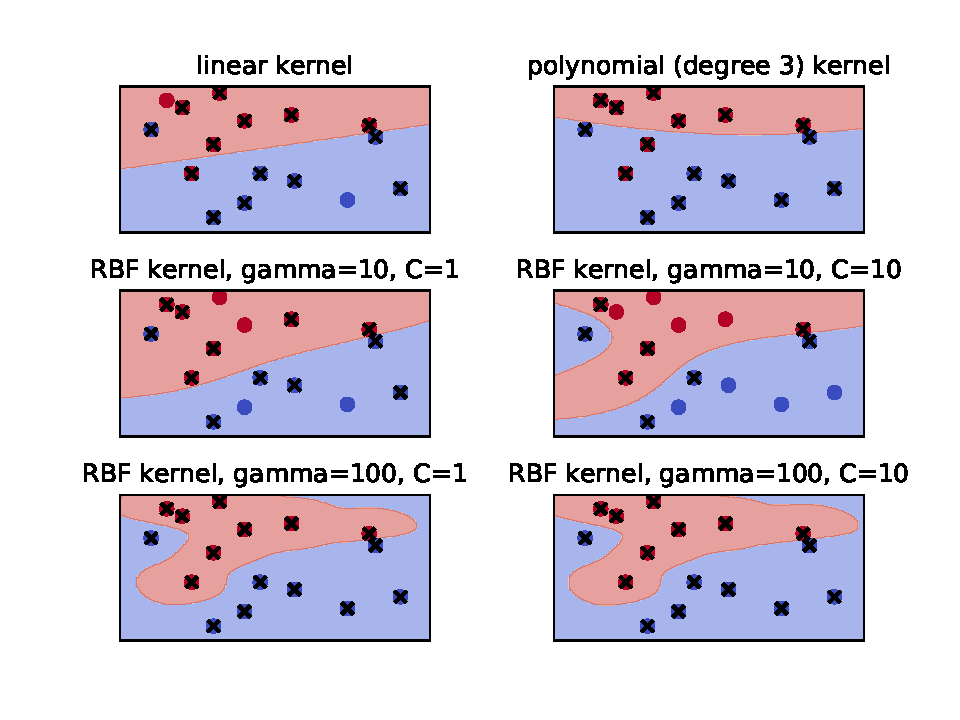
\includegraphics[scale=0.7]{figure.pdf}
\caption{Support Vectors}
\end{figure} 
The support vectors are marked with "X". \\
Through observation,  the C parameter determines "the relative importance between large margin and small total price($\sum \xi _i$)", which invokes the trade-off between training-error penalty and stability.  A large C provides low bias and high variance and vice versa.
Another parameter $\gamma \propto \frac{1}{\sigma^2}$ intuitively implies the influence range of a single support vector. (i.e.  large $\gamma \rightarrow$ small variance  $\rightarrow$ the support vector does not have wide-spread influence." ) According to the documentation, lower $\gamma$ leads to smoother models and large $\gamma $ may lead to overfitting.
\footnote{Reference: \url{http://scikit-learn.org/stable/auto_examples/svm/plot_rbf_parameters.html\#sphx-glr-auto-examples-svm-plot-rbf-parameters-py}} 
% Usually, low $\gamma$ leads to low bias and high variance while large $\gamma$ leads to higher bias and low variance. WRONG??
When $\gamma$ and $C$ are small, the RBF kernel is able to simulate linear kernel.
\end{solution}
\end{document}